%At this point we already know that an UPPAAL scheme resembles a probabilistic model.  
%
A location may have many outgoing edges, in which only 1 edge must be taken at a time. 
%
This feature is only possible with the use of branch points, that coordinate all outgoing edges of a location based on a probabilistic value.
%
%and to also eliminate redundant locations. 
%
In this chapter we will explain how a probabilistic model scheme is constructed, from the integration of the fitted equations obtained from all analyses.

\section{Final Analysis Processing}
%
After completing the analyses of each trace obtained from a model simulation, the results are gathered in a list of $Analysis$ objects. 
%
The way that the results are handled is described in Algorithm \ref{finalAnalysis}. 
%
Given a stack of equations obtained from the function fitting algorithms, a new template is created for each different variable that is found.
%
If a template for a variable was already created, this last one is only updated.
%
Each equation retrieved from the stack is represented as a location, that is integrated in the final probabilistic model. 
%
The procedure of how branch points, edges and locations are connected to each other is explained in the next sections. 
%

\input{./algorithms/UPPAAL/UPPAALAlgorithm.tex}

\section{Creating Locations}
The $equationStack$ parameter of Algorithm \ref{joinLocations}, contains all of the fitted equations of a trace.
%
A new location with an invariant and a self-pointing edge is created, based on the information of each equation obtained from the stack.
%
Before connecting the new location to a component of the template, we first reference a branch point (variable $branchPoint$) that is already integrated in the template.
%
As previously mentioned, every template is initialized with an initial-urgent location called $Start$, that has an outgoing edge leading to the initial branch point called $BP$. 
%
The variable $branchPoint$ always references $BP$ every time the first equation from a stack is retrieved.
%
Otherwise, $branchPoint$ references the outgoing branch point of the previous location that was attached to the model. 
%
In case that a previous location has no outgoing branch point, then a new one is created and attached to it.
%
The $previousLocation$ variable always refers to the last location that was added to the template.
%
The method $probabilityModelling$ is the one that actually incorporates a new location to the template and returns a reference of it. 
%
In order to keep consistency and efficiency of the constructed probabilistic model, 5 cases must be considered before adding a new location to a template. 
%
The explanation of the $probabilityModelling$ method is shown on the next section. 

\input{./algorithms/UPPAAL/JoinLocationsAlgorithm.tex}

\section{Probabilistic Modelling}
The $probabilityModelling$ method consists of first verifying the functionality of the new location that is going to be added to the template, before attaching it to any branch point (as seen in Algorithm \ref{Probability-Modelling}). 
%
We begin by first performing an inspection of the outgoing edges that the current branch point ($branchPoint$) already possesses (if any). 
%
The $equation$ variable references the equation of an outgoing location ($location$) of $branchPoint$, that is already incorporated in the template.
%
The $newEquation$ variable references the equation of the new location ($newLocation$) that is going to be incorporated in template. 
%
If the fitted functions (or $data$ attributes) from $equation$ and $newEquation$ are equal, it means that there exists a location in the template with the same functionality as the new location to be incorporated. 
%
Whenever this happens, we proceed and verify the time duration of both equations.
%
The $newLocation$ might be added to the model, depending on the difference of time duration between the two equations. 
%
%The method $processEquationData$ modifies the current template based on the equations of the locations that are given as parameters, and returns the reference of the last updated location of the template.
%
There are five possible scenarios that can occur when analyzing the equations of a trace in method $processEquationData$, which are explained in Sections \ref{Case 1} - \ref{Case 5} (Notice that $EQ$ is the equation of $location$ and $EQ'$ the one from $newLoc$). 
%
Whenever $branchPoint$ has no edges pointing to other locations with the same functionality as $newLocation$, then a new outgoing edge is added to $branchPoint$ that leads to $newLocation$. 
A probabilistic model is created after Algorithm \ref{Probability-Modelling} terminates, which represents the recreated model that describes the trending of the data from the traces that were analyzed. The verification of the similarities and differences between the recreated model and the original one are discussed in the next chapter. 
\\
\\
\input{./algorithms/UPPAAL/ProbabilityModellingAlgorithm.tex}
%
%\input{./algorithms/UPPAAL/PrePosProcessAlgorithm.tex}

\subsection{Case 1 (Identical Equations)} \label{Case 1}
If both of the equations start and end at the same time, it means that both of them are identical (Fig 7.1).
%
In this case $newLoc$ is deleted from the template and the edge that leads to $location$ is incremented by 1. 
%
The returned location is $location$.

%\centering
\begin{figure}[b]
%	\label{Case 1}
	\centering
	%	\label{fig:practical-example}
	\begin{tabular}{cc}
		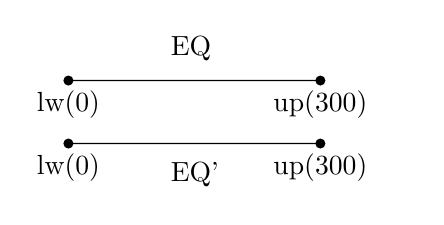
\begin{tikzpicture}[scale=0.8]
		\filldraw 
		(0,0) circle (2pt) node[align=left,   below] {lw(0)} --
		(4,0) circle (2pt) node[align=center, below] {up(300)};
		\node[text width=3cm] at (3.5,1.5) {EQ};
		\newline
		
		\filldraw 
		(0,1) circle (2pt) node[align=left,   below] {lw(0)} --
		(4,1) circle (2pt) node[align=center, below] {up(300)};
		\node[text width=3cm] at (3.5,-0.5) {EQ'};
		\end{tikzpicture}&
		\includegraphics[scale=0.8]{./pictures/Bpcases/case1.PNG}
	\end{tabular}
\caption{Example of the addition of the same equation to a model}
\end{figure}

%\caption{Case 1}
%\end{figure}

\subsection{Case 2 (Same Starting-Time Equations)}
Both equations start at the same time, but end at different ones (Fig 7.2). 
%
Location $newLoc$ is added to the model with a slight modification of its time bounds.
%
Its lower bound remains the same, but the upper bound is updated to the smallest $upperBound$ value from the two equations $EQ$ and $EQ'$.
%
The location returned for both cases 2a) and case 2b) is $newLoc$.
\\
\\
\begin{figure}[t]

	%	\label{fig:practical-example}
	\centering
	\begin{tabular}{cc}
		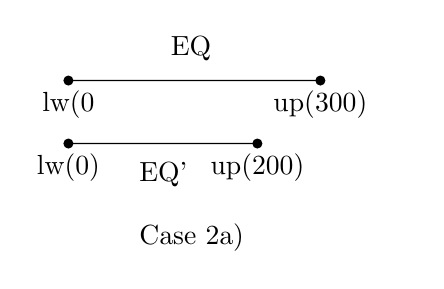
\begin{tikzpicture}[scale=0.8]
		\filldraw 
		(0,0) circle (2pt) node[align=left,   below] {lw(0)} --
		(3,0) circle (2pt) node[align=center, below] {up(200)};
		\node[text width=3cm] at (3.5,1.5) {EQ};
		\newline
		
		\filldraw 
		(0,1) circle (2pt) node[align=left,   below] {lw(0} --
		(4,1) circle (2pt) node[align=center, below] {up(300)};
		\node[text width=3cm] at (3,-0.5) {EQ'};
		
		\node[text width=3cm] at (3,-1.5) {Case 2a)};
		\end{tikzpicture}&
		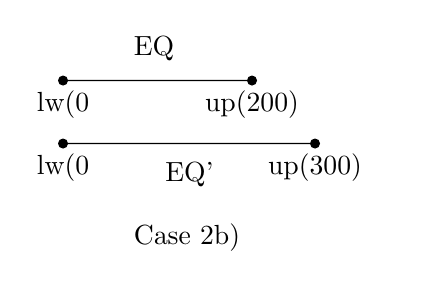
\begin{tikzpicture}[scale=0.8]
		\filldraw 
		(0,0) circle (2pt) node[align=left,   below] {lw(0} --
		(4,0) circle (2pt) node[align=center, below] {up(300)};
		\node[text width=3cm] at (3,1.5) {EQ};		
		\newline
		
		\filldraw 
		(0,1) circle (2pt) node[align=left,   below] {lw(0} --
		(3,1) circle (2pt) node[align=center, below] {up(200)};
		\node[text width=3cm] at (3.5,-0.5) {EQ'};
		
		\node[text width=3cm] at (3,-1.5) {Case 2b)};
		\end{tikzpicture} 
	\end{tabular}
	
	\begin{tabular}{c}
		\includegraphics[scale=0.8]{./pictures/Bpcases/case2.PNG}
	\end{tabular}
	\caption{Example of the addition of an equation that begins at the same time to a model}
\end{figure}


\subsection{Case 3 (Same Ending-Time Equations)}
Both equations begin at different times, but finish at the same one (Fig 7.3). 
%
The new location $newLoc$ is introduced in the model with a slight modification of its time bounds.
%
Its lower bound is updated to the $lowerBound$ from the equation that has more time duration among $EQ$ and $EQ'$.
%
The upper bound is updated to the $lowerBound$ of the equation with the smallest duration time. 
%
Once $newLoc$ is integrated in the model, $location$ is updated by setting its $lowerBound$ to the $upperBound$ of $newLoc$. 
%
The returning location for both cases 3a) and 3b) is always $newLoc$.
\\
\\
\begin{figure}[h]
	\centering
	%	\label{fig:practical-example}
	\begin{tabular}{cc}
		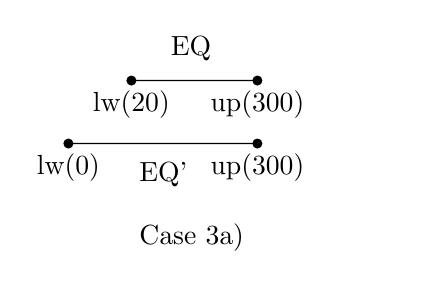
\begin{tikzpicture}[scale=0.8]
		\filldraw 
		(0,0) circle (2pt) node[align=left,   below] {lw(0)} --
		(3,0) circle (2pt) node[align=center, below] {up(300)};
		\node[text width=3cm] at (3.5,1.5) {EQ};
		\newline
		\filldraw 
		(1,1) circle (2pt) node[align=left,   below] {lw(20)} --
		(3,1) circle (2pt) node[align=center, below] {up(300)};
		\node[text width=3cm] at (3,-0.5) {EQ'};
		
		\node[text width=3cm] at (3,-1.5) {Case 3a)};
		\end{tikzpicture}&
		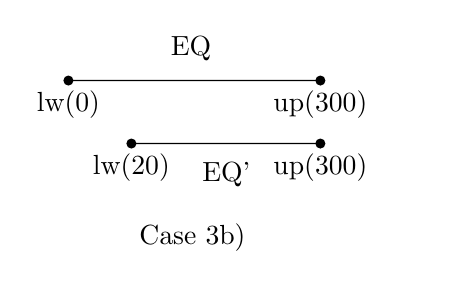
\begin{tikzpicture}[scale=0.8]
		\filldraw 
		(1,0) circle (2pt) node[align=left,   below] {lw(20)} --
		(4,0) circle (2pt) node[align=center, below] {up(300)};
		\node[text width=3cm] at (3.5,1.5) {EQ};
		\newline
		\filldraw 
		(0,1) circle (2pt) node[align=left,   below] {lw(0)} --
		(4,1) circle (2pt) node[align=center, below] {up(300)};
		\node[text width=3cm] at (4,-0.5) {EQ'};
		
		\node[text width=3cm] at (3,-1.5) {Case 3b)};
		\end{tikzpicture} 
	\end{tabular}
	
	\begin{tabular}{c}
		\includegraphics[scale=0.8]{./pictures/Bpcases/case3.PNG}
	\end{tabular}
	\caption{Example of the addition of an equation that ends at the same time to a model}
\end{figure}

\newpage
\subsection{Case 4 (Contained Equations)}
In this scenario, an equation has a time duration that is a sub-interval of the time duration of the other equation (Fig 7.4).  
%
The new location $newLoc$ is introduced in the model with a slight modification of its time bounds.
%
Its lower bound is updated to the $lowerBound$ from the equation with the highest duration time.
%
The upper bound is updated to the $lowerBound$ of the equation with the lowest duration time. 
%
Once $newLoc$ is integrated to the model, it now requires 2 outgoing edges. 
%
The first outgoing edge must go to a location with the $upperBound$ of $EQ$, while the other must go to another location with the $upperBound$ of $EQ'$. 
%
The returning location for both cases 4a) and 4b) is $newLocation$.
\\
\\
\begin{figure}[h]
	\centering
	%	\label{fig:practical-example}
	\begin{tabular}{cc}
		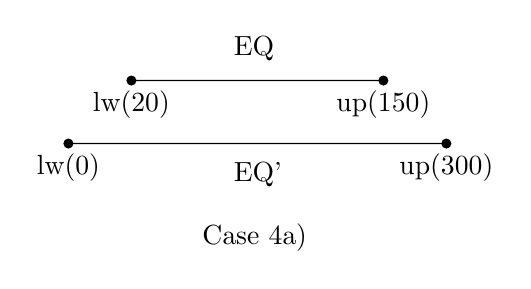
\begin{tikzpicture}[scale=0.8]
		\filldraw 
		(-1,0) circle (2pt) node[align=left,   below] {lw(0)} --
		(5,0) circle (2pt) node[align=center, below] {up(300)};
		\node[text width=3cm] at (3.5,1.5) {EQ};
		\newline
		\filldraw 
		(0,1) circle (2pt) node[align=left,   below] {lw(20)} --
		(4,1) circle (2pt) node[align=center, below] {up(150)};
		\node[text width=3cm] at (3.5,-0.5) {EQ'};
		
		\node[text width=3cm] at (3,-1.5) {Case 4a)};
		\end{tikzpicture}&
		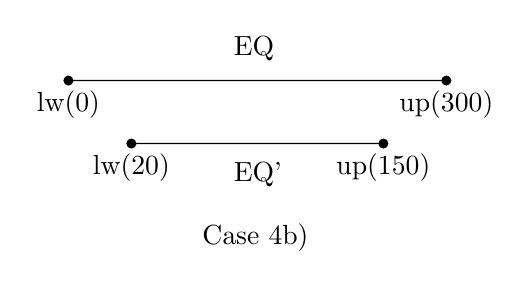
\begin{tikzpicture}[scale=0.8]
		\filldraw 
		(-1,1) circle (2pt) node[align=left,   below] {lw(0)} --
		(5,1) circle (2pt) node[align=center, below] {up(300)};
		\node[text width=3cm] at (3.5,1.5) {EQ};
		\newline
		\filldraw 
		(0,0) circle (2pt) node[align=left,   below] {lw(20)} --
		(4,0) circle (2pt) node[align=center, below] {up(150)};
		\node[text width=3cm] at (3.5,-0.5) {EQ'};
		
		\node[text width=3cm] at (3,-1.5) {Case 4b)};
		\end{tikzpicture}
	\end{tabular}
	
	\begin{tabular}{c}
		\includegraphics[scale=0.8]{./pictures/Bpcases/case4.PNG}
	\end{tabular}
	\caption{Example of the addition of an equation with a sub-interval of time to a model}
\end{figure}
\newpage
\subsection{Case 5 (Continued Equations)}\label{Case 5}
Here an equation begins right after the previous one finished (Fig 7.5). 
%
The new location $newLoc$ is only added as an outgoing edge of the location that was already in the model ($location$).
%
The returning location in this case is always $newLoc$. 
\\ 
\\
\begin{figure}[b]
	\centering
	%	\label{fig:practical-example}
	\begin{tabular}{cc}
		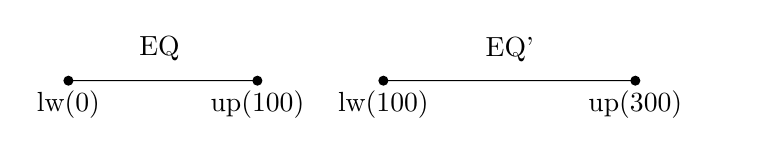
\begin{tikzpicture}[scale=0.8]
		\filldraw 
		(0,0) circle (2pt) node[align=left,   below] {lw(0)} --
		(3,0) circle (2pt) node[align=center, below] {up(100)};
		\node[text width=3cm] at (3,0.5) {EQ};
		\newline
		
		\filldraw 
		(5,0) circle (2pt) node[align=left,   below] {lw(100)} --
		(9,0) circle (2pt) node[align=center, below] {up(300)};
		\node[text width=3cm] at (8.5,0.5) {EQ'};
		\end{tikzpicture}&
		
	\end{tabular}
	
	\begin{tabular}{c}
		\includegraphics[scale=0.8]{./pictures/Bpcases/case5.PNG}
	\end{tabular}
	\caption{Example of the addition of an equation that starts at the ending time of another equation to a model}
\end{figure}

%\newpage
%A probabilistic model is created after Algorithm \ref{Probability-Modelling} terminates, which represents the recreated model that describes the trending of the data from the traces that were analyzed. The verification of the similarities and differences between the recreated model and the original one are discussed in the next chapter. 



